We advocate for a strong coupling between model and source-code, to give architects and developers a way to both interact during the whole development cycle. PAMELA is an annotation-based Java modeling framework providing a smooth integration between model and code, without code generation nor externalized model serialization. The idea is to avoid separation between modeling and code to facilitate consistency management and to /avoid round-trip issues. Figure \ref{fig:PamelaVision} summarizes the PAMELA architecture.  

\begin{figure}
    \centering
    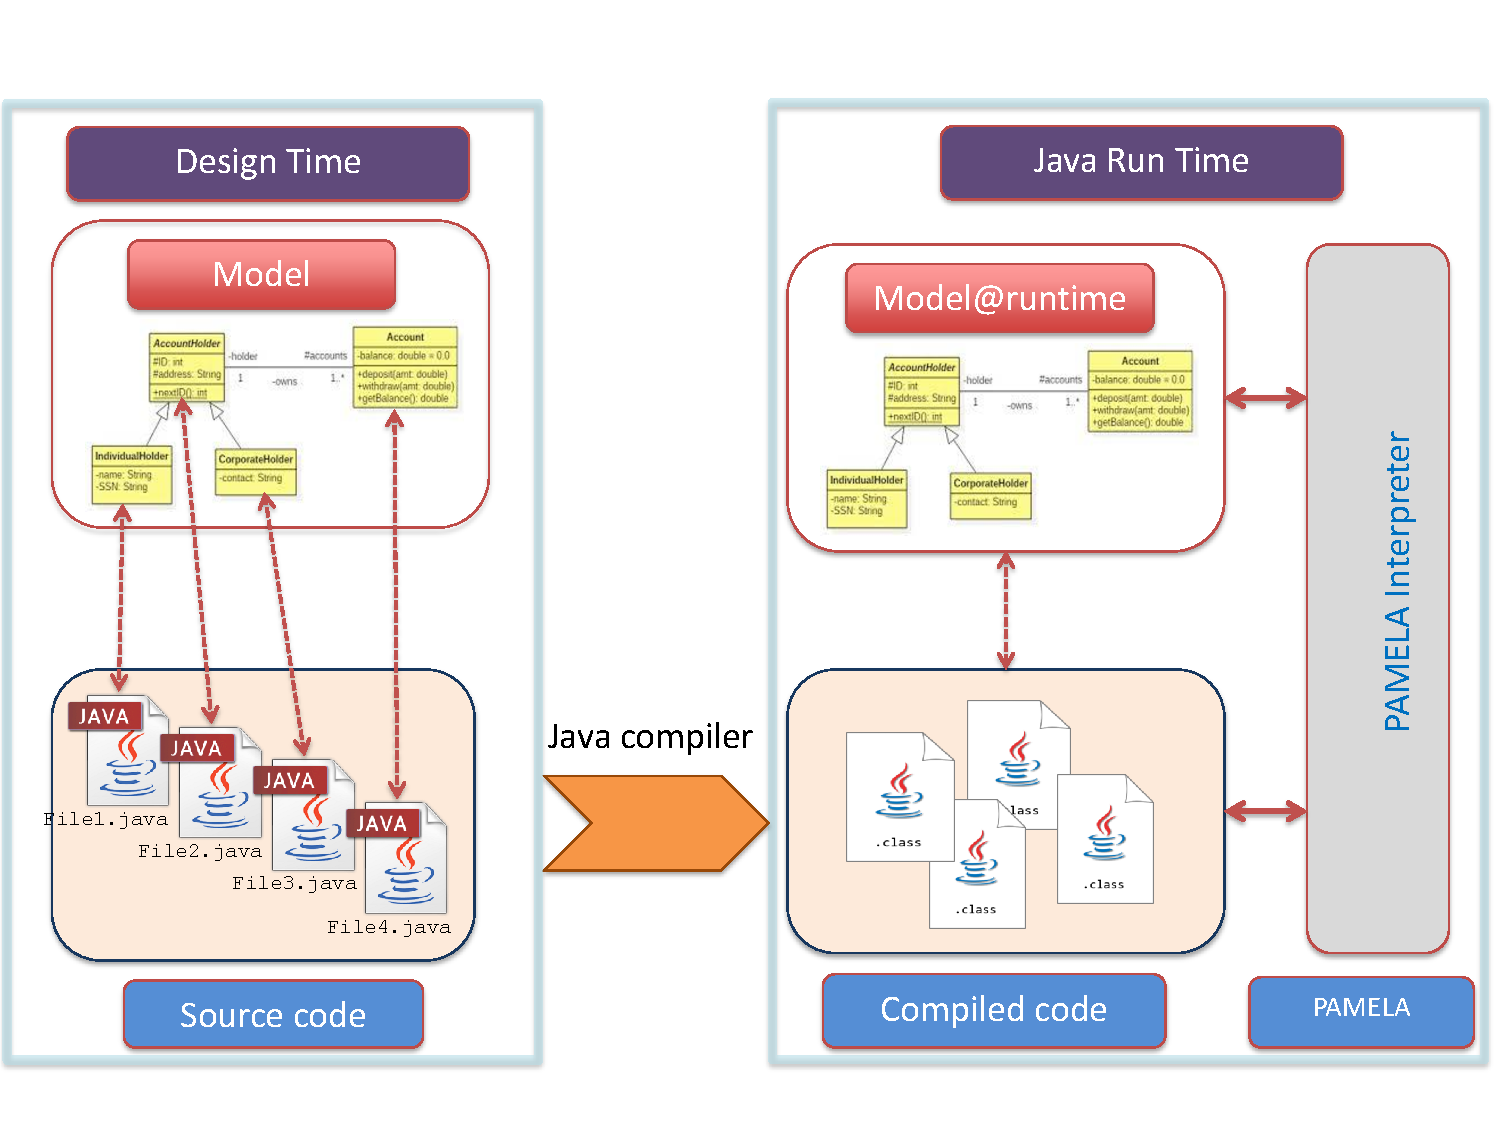
\includegraphics[width=1.0 \columnwidth]{PamelaVisionV2.pdf}
    \caption{PAMELA approach for modelling}
    \label{fig:PamelaVision}
\end{figure}

%\subsection{PAMELA Modeling/Development Process}

Coupling model and code into the same artifact opens new ways of programming. The classical (metadata enabled) programming process relies on \emph{programmers} that produce code reusing pre-existing modeling concepts. These concepts are implemented by \emph{modelers} that provide the right annotations the programmers use. This is, for instance, the process followed by Jakarta EE (JEE) developers reusing JEE specific annotations. The evolution rhythm between models and code is low. This programming way is still possible with PAMELA, but we allow the ability to reach a high evolution rhythm when the programmer also becomes the modeler. In fact, when a pattern, an abstraction, a generalization is identified by the programmer, s/he can use PAMELA to develop and capitalize on this abstraction by increasing PAMELA metamodel. 

% Je pense qu'ici il faudrait plutot parler du modèle. Le métamodèle PAMELA est celui représenté figure 3. Ou alors parler du metametamodele PAMELA

The developed metamodels are implemented by annotations that rely on Java/JVM entities and mechanisms. They include consistency checkings, which constrain their use and helps the programmer to avoid inconsistencies or errors. We have first experimented their use with setter/getter to define POJO entities, with traits to implement multiple inheritance or with roles and rules to set security rules on classes.

Our experience shows that introducing and reusing new concepts (1) reduce the size of the code, (2) reduce the risk of errors and (3) improve the code structure. The cycle of development between the model and the code can then be drastically reduced, leading to what we call \emph{continuous modeling}.

The code size is reduced because abstractions factorize recognized concepts so that the code using such concepts is replaced by the use of the abstraction at the right place. This also reduces the risk of errors since the code is now managed by the PAMELA framework with all the required checks. Finally, the code structure is improved since it matches the way the programmer conceptualizes (models) her/his code.

\ab{In this presentation, we focus on the programming use of PAMELA, when programmers reuse existing annotations. The full power of PAMELA arises when programmers become modelers defining their own abstractions/annotations.} 

